\documentclass{standalone}

\usepackage[OT1]{fontenc}
\renewcommand*\familydefault{\sfdefault}
\usepackage{helvet,sfmath}
\usepackage{siunitx}

\usepackage{tikz}
\usetikzlibrary{arrows,calc,patterns}
\usetikzlibrary{intersections, calc, arrows.meta}
\usepackage{tikz,tkz-euclide}

\definecolor{Diverging_Lens}{RGB}{148,122,255}
\definecolor{Converging_Lens}{RGB}{255,62,155}
\definecolor{Light}{RGB}{255,190,71}
\definecolor{Note}{RGB}{86,39,255}



\begin{document}

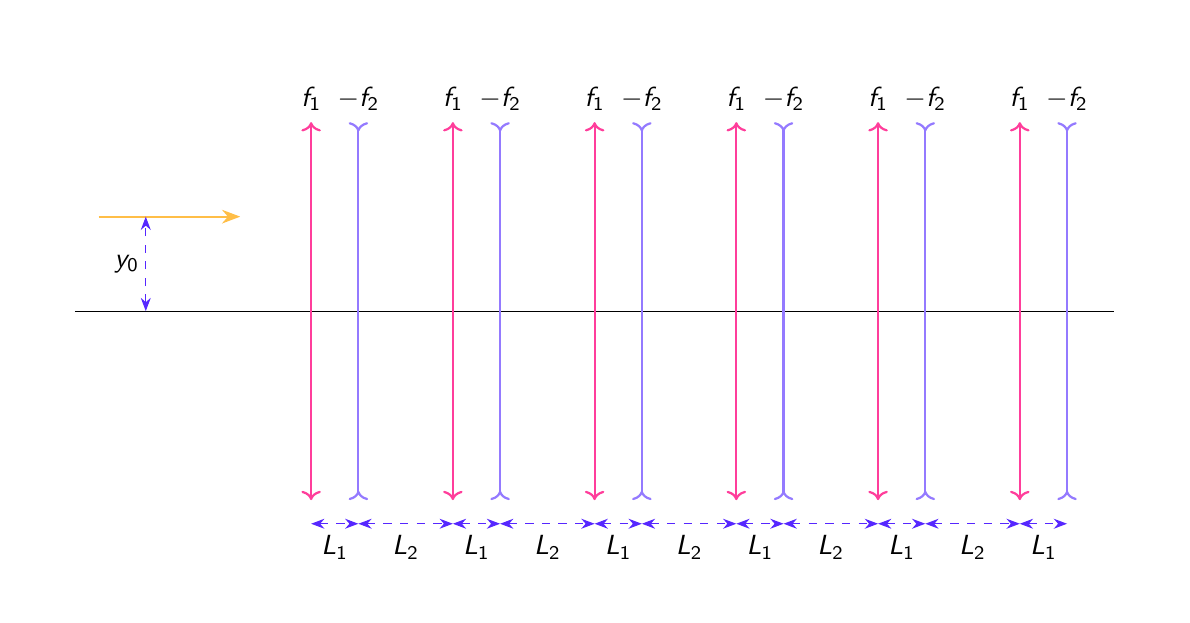
\begin{tikzpicture}[scale=0.6]
    %% Background
    \draw[draw=none] (-12,-6) to (-12,6) to (12,6) to (12,-6) to (-12,-6);

    %% Optics Axis
    \draw (-11,0) to (11,0);

    %% Lens
    \foreach \x in {-6,-3,0,3,6,9}
    {
        \draw[Converging_Lens, thick,<->] (\x,-4) to (\x,4);
        \draw[Diverging_Lens, thick, >-<] (\x+1,-4) to (\x+1,4);
        \draw 
        (\x,4.5) node{\(f_1\)}
        (\x+1,4.5) node{\(-f_2\)}
        ;
        \draw[Note, dashed, Stealth-Stealth] (\x,-4.5) to (\x+1,-4.5);
        \draw (\x+0.5,-5) node{\(L_1\)};
    }
    \foreach \x in {-6,-3,0,3,6}
    {
        \draw[Note, dashed, Stealth-Stealth] (\x+1,-4.5) to (\x+3,-4.5);
        \draw (\x+2,-5) node{\(L_2\)};
    }

    %% Light
    \draw[Light, thick, -Stealth] (-10.5,2) to (-7.5,2);
    \draw[Note, dashed, Stealth-Stealth] (-9.5,0) to (-9.5,2);
    \draw (-9.9,1) node{\(y_0\)};
\end{tikzpicture}

\end{document}
